\documentclass{article}
\usepackage{graphicx}
\usepackage{float}% Required for inserting images

\title{Introducción al Analisis de Datos: Actividad 2}
\author{Gabriel Freire Parola, Matias Cabello, Jonathan Suarez, \\ Santiago Seleme, Santiago Llugany }
\date{October 2025}

\begin{document}

\maketitle

\section*{Modelo de POO de un Auto con instancias auto1 y auto2}
\begin{figure}[H]
    \centering
    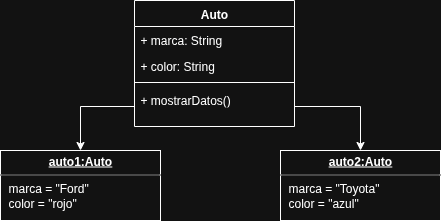
\includegraphics[width=1\linewidth]{diagrama_UML.png}
    \caption{Modelo UML}
    \label{fig:placeholder}
\end{figure}
\begin{figure}[H]
    \centering
    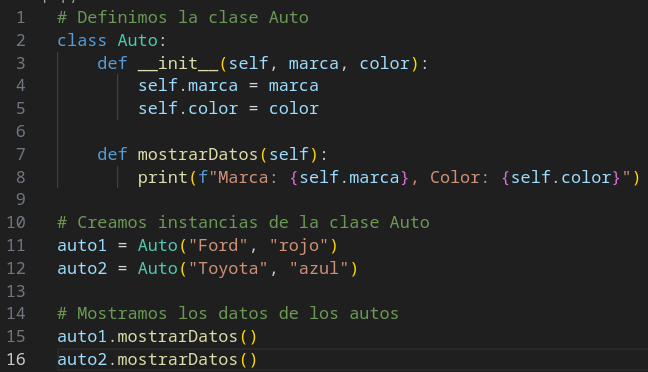
\includegraphics[width=0.5\linewidth]{codigo.png}
    \caption{El modelo en un script Python}
    \label{fig:placeholder}
\end{figure}
\begin{figure}[H]
    \centering
    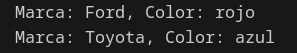
\includegraphics[width=0.5\linewidth]{ejecucion.png}
    \caption{Ejecución donde se muestran los datos de las dos instancias.}
    \label{fig:placeholder}
\end{figure}
\textbf{Una instancia es un objeto particular creado a partir de una copia especifica de la clase con valores propios para sus atributos.}
\end{document}
